\documentclass[12pt,letterpaper]{article}
\usepackage{anysize}
\usepackage{graphicx}
\usepackage{hyperref}

\marginsize{2cm}{2cm}{1cm}{1cm}
\begin{document}

\title{Noise Based World/Island Generation (Final Project)}
\author{Benjamin Friedman\\
friedmab@oregonstate.edu\\
CS 557\\
\url{https://media.oregonstate.edu/media/t/0_2h44f2sm}\\
}

\maketitle

\centerline{
	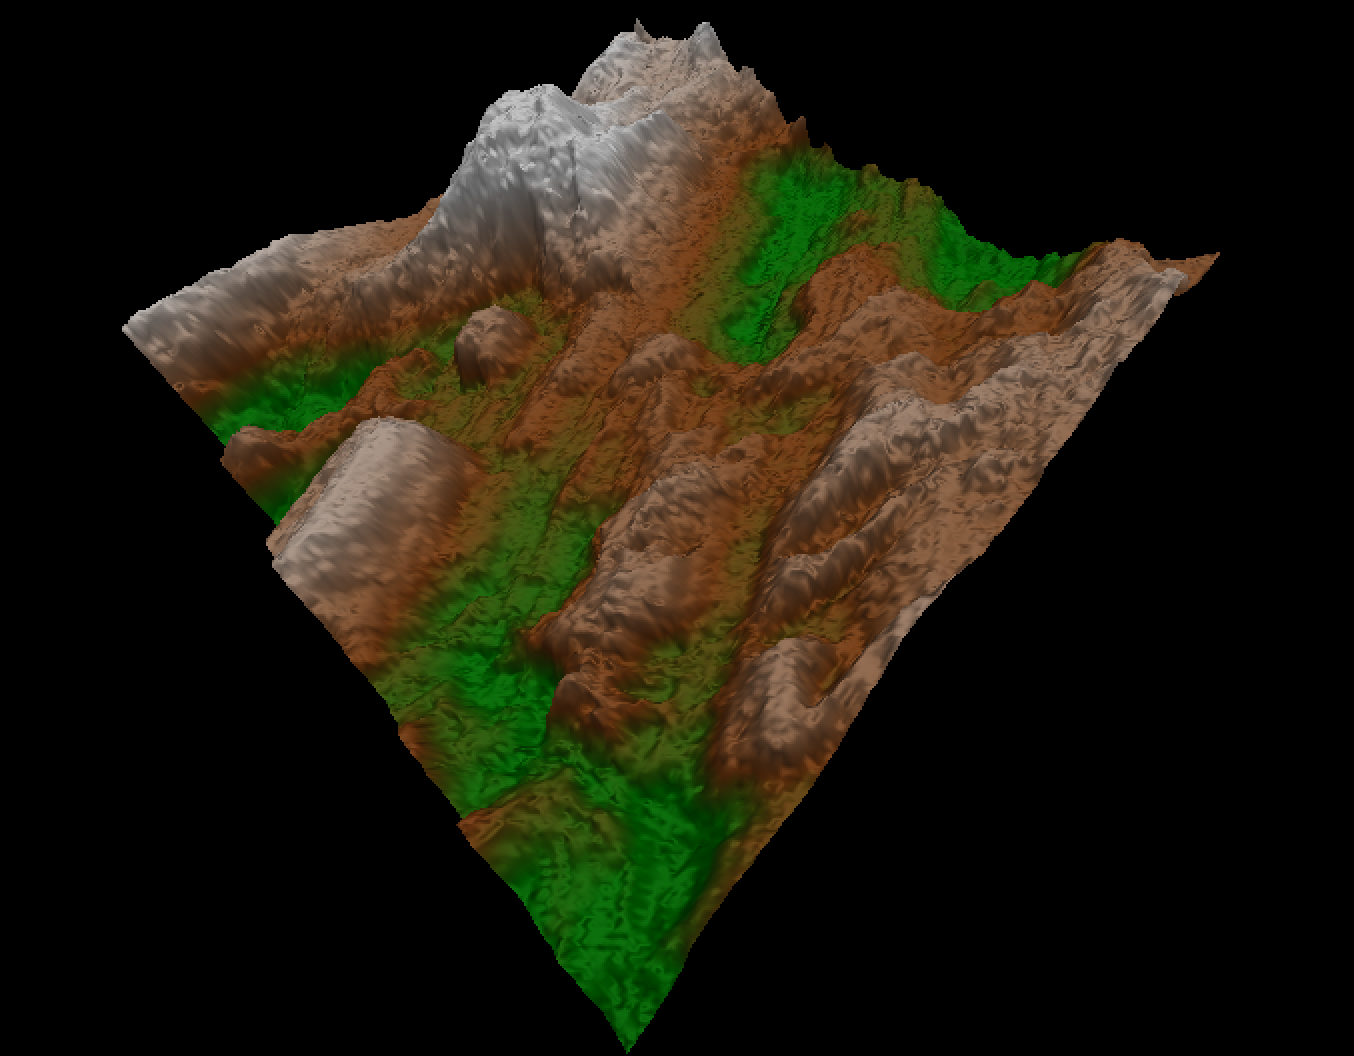
\includegraphics[width=0.51\textwidth,keepaspectratio]{./p1}
	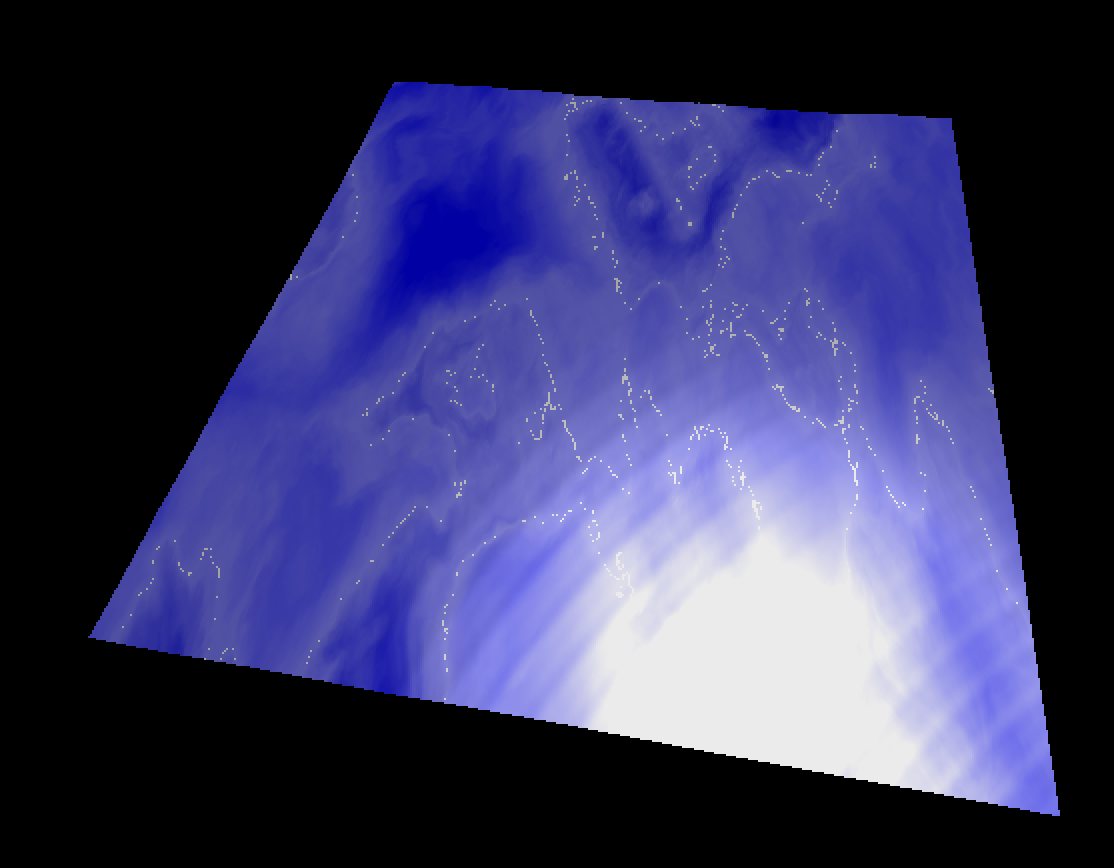
\includegraphics[width=0.51\textwidth,keepaspectratio]{./p2}
}

\centerline{
	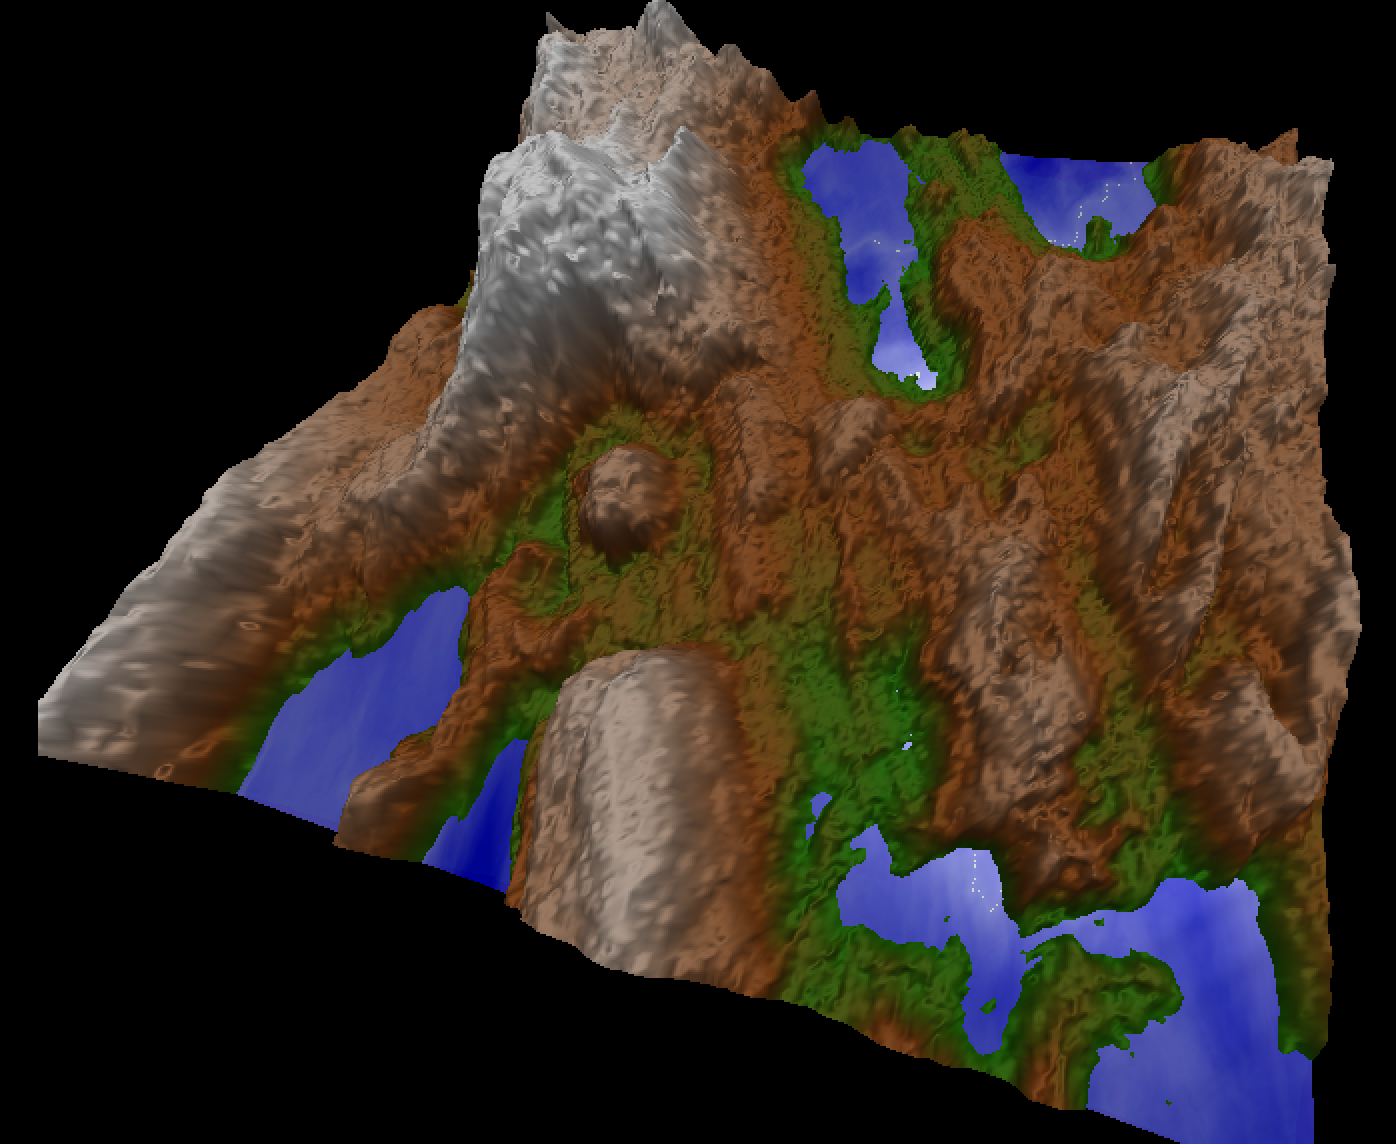
\includegraphics[width=0.51\textwidth,keepaspectratio]{./p3}
	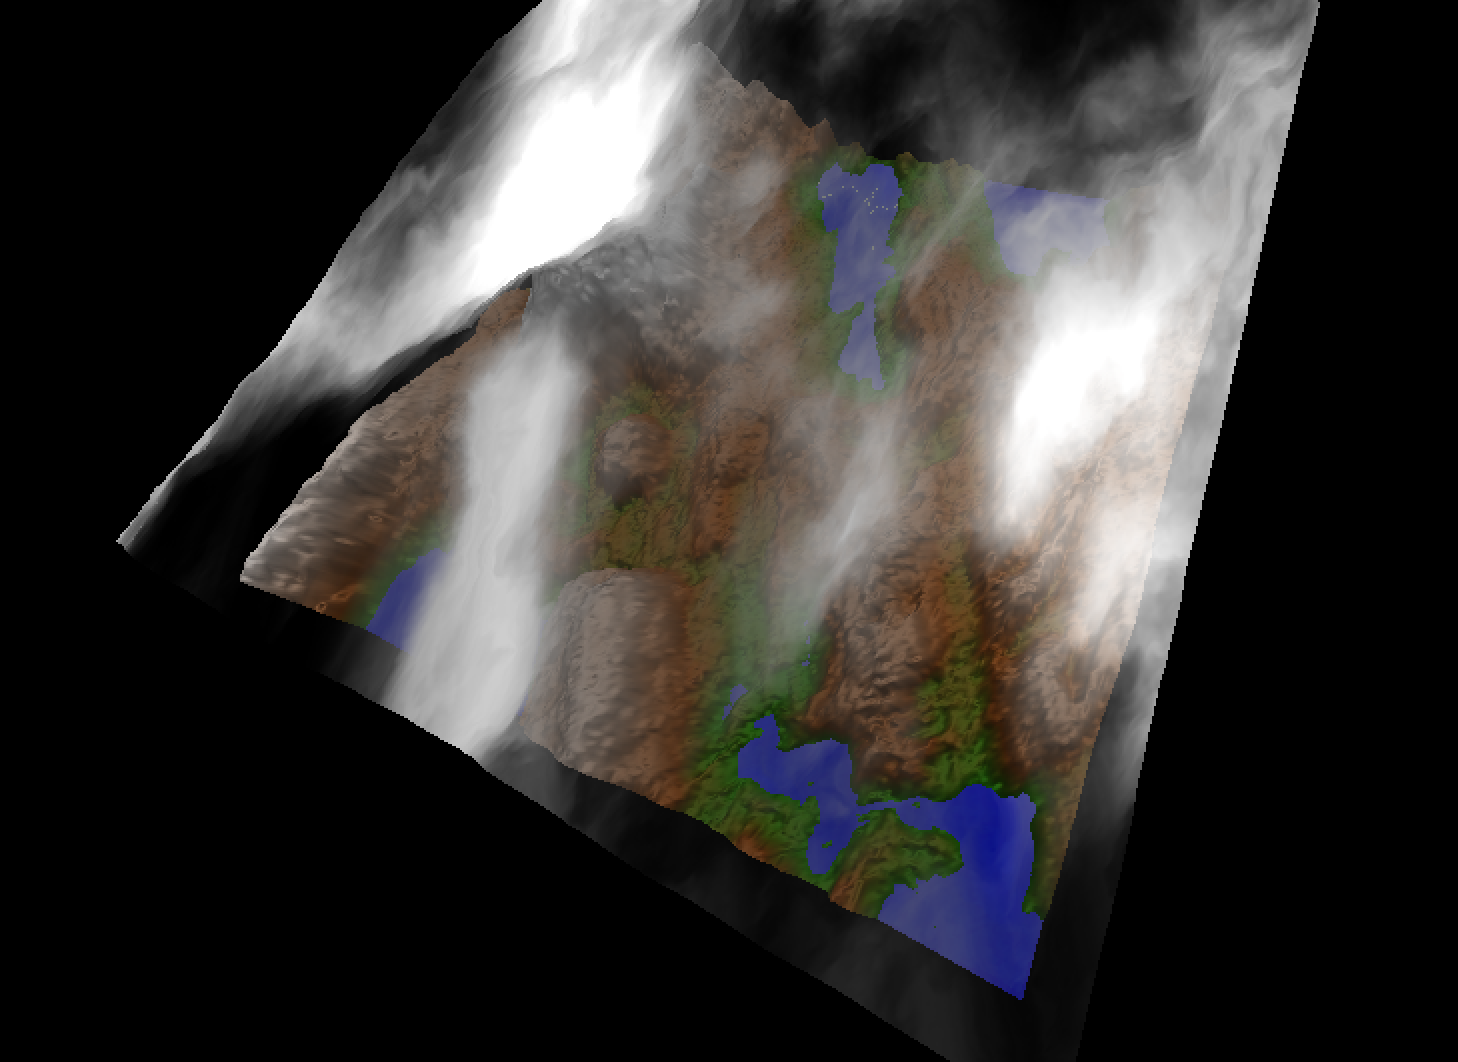
\includegraphics[width=0.51\textwidth,keepaspectratio]{./p7}
}

% what you did and explaining why it worked this way
In this project I implemented noise based world generation purely in shaders. To setup the world to generate I proceeded to lay out 3 different quads, one for water, one for land, and one for the clouds. For each of these I utilized a hash function to compute values from 4 different 'tile' sections for any given S and T (or X and Z) pair, and the resultant values were then used to interpolate a given value value across the tile. This process was integrated into a fractal brownian noise ($fbm$) implementation, which utilized repeated octaves with increasing frequency (and decreasing  amplitude) to greatly increase the detail over time \cite{fractional_brownian_motion}. This noise generation was done purely in OpenGL Shading Language, taking only an initial seed to shift the results slightly from iteration to iteration.


To produce a more interesting fractal I took the $fbm$ of the $fbm$ of the $fbm$ ($fpm^3$) of the initial input value \cite{shader_book}. This resulted in a deeper fractal, and more realistic looking results. For the terrain generation this fractal result was utilized to generate a height map, which was then color coded by the height position within the world. For the water, $fbm$ was used to produce a subtle flowing effect within itself, along with a white ridge (a crest of water) along median values. A decreased amplitude $fbm$ was applied to slightly deform the water sheet and to give some slight undulation, and a pair of sine waves were applied to slightly adjust the normal and produce a ripple effect via bump-mapping.


Finally, the clouds themselves were computed by applying $fpm^3$ to create a very smooth, and fluffy looking cloud cover. Values produced by $fpm^3$ were discarded below a certain value, and values above were gradually increased in RGBA by a factor of 3.0. This caused small white values to remain relatively small, and transparent, but to quickly ramp up in opacity and brightness as the values increased slightly. This gave them a visual appearance of cumulus clouds, but without the vertical component \cite{clouds}.


Because all of these elements were based off of the same underlying $fbm$ values (with alterations to each domain of land, sea, and air), I was able to additionally get an effect of clouds hanging around the mountains, which looked quite realistic. In addition, I was able to add in an extra $fbm$ function to both the water and land shaders which computed the exact same $fbm$ values as the cloud shader. The result was that I was able to apply shadows across the water and land as the clouds moved overhead. To cap this all off, per-fragment lighting was used, and the location of the light was setup on a toggle to rotate around the world in a day-night cycle.


Compared to my original proposal, this does everything which was mentioned before. Some slight changes included the water being a calmer representation (as it ended up being landlocked and needed to look more placid), and adding the cloud shadows across the landscape.


\begin{thebibliography}{9}

\bibitem{shader_book}
Gonzalez, Patricio. Lowe, Jen. "Fractal Brownian Motion". \textit{The Book of Shaders}. 2015. https://thebookofshaders.com/13/. Accessed: March 1st, 2020.

\bibitem{job_talle}
Talle, Job. "Cubic Noise". \textit{Job Talle}. Oct. 31s, 2017. https://jobtalle.com/cubic\_noise.html. Accessed: Feb. 24th, 2020.

\bibitem{fractional_browning_motion}
Ndaoud, Mohamed. "Constructing the fractional Brownian motion". \textit{Institut des Hautes Etudes Scientifiques}. May 18th, 2017. https://www.youtube.com/watch?v=XXSCwm06J\_w. Accessed: March 14th, 2020.

\bibitem{ocean_sim}
Alekseev, Alex. "Seascape". \textit{Shadertoy}. Sept. 26th, 2014.  https://www.shadertoy.com/view/Ms2SD1. Accessed: Feb. 28th, 2020.

\bibitem{fire_sim}
Duprat, Anatole. "Flame". \textit{Shadertoy}. Feb. 15th, 2013. https://www.shadertoy.com/view/MdX3zr. Accessed: Feb. 28th, 2020.

\bibitem{clouds}
UCAR. "Cumulus Clouds". \textit{UCAR: University Corporation for Atmospheric Research}. Jan. 7th, 2020. https://scied.ucar.edu/imagecontent/cumulus-clouds. Accessed: March 14th, 2020.

\end{thebibliography}


\end{document}
